% Part 2 chapter carrying "A Note on Entropic Gravity and the Thermodynamic-Gravity Conjecture" (March 2026, 10 pp) in its order and words.
% Read in full 2026-10-03 (PDF text 317 lines with page markers, ledger docs/book/PAPER_LINE_COUNTS.md row 5); LaTeX base IAM_Saridakis_Bridge.tex.
% Corrections applied: docs/verification/PAPER_ERRATA.md EG1-EG8; docs/verification/theory/ENTROPIC_GRAVITY_NOTE_CHECK.md; published abstracts
% (Luciano 2025, DESI 2024 VII, Andrade 2024) for the data quoted. Numbers: docs/verification/scripts/verify_entropic_gravity.py (+ _output.txt).
% Figure: docs/book/figscripts/fig_p2_entropic_gravity.py. Summary of the same comparison in Chapter ch:theory, Section sec:source.
\chapter{Entropy law or entropy source: the thermodynamic-gravity conjecture}\label{ch:entropicgravity}

\section*{The question}
A family of cosmologies starts from one result: the Friedmann equations follow from the first law of thermodynamics applied to the cosmic horizon. The
family then divides over one question. Does new physics enter through the entropy law of the horizon, or through an entropy source that the law had not
counted? Chapter~\ref{ch:theory} (Section~\ref{sec:source}) stated the answer IAM gives in one paragraph. This chapter sets out the comparison in full: the
shared starting point, the two roads from it, where each leads, the coupling constant, the activation function, the two families side by side, and the
predictions that separate them.

IAM is not a rival to general relativity. It keeps the Bekenstein--Hawking area law exactly and counts the Landauer cost of the records that matter
writes as it decoheres, written to the nearest surface --- here the cosmic horizon.

% ============================================================
\section{The shared starting point}\label{sec:eg_start}
IAM begins from the same foundation as holographic dark energy models in the Barrow--Tsallis tradition: the \emph{thermodynamic-gravity conjecture}. In this
framework the standard Friedmann equations governing cosmic expansion are not fundamental --- they are thermodynamic equations of state derivable from the
first law of thermodynamics applied to the cosmic horizon. \interp

The derivation proceeds through the Cai--Kim formalism~\cite{CaiKim2005}. In a flat Friedmann--Robertson--Walker universe the apparent horizon has radius
$\tilde r_A=1/H$, area $A_H=4\pi/H^2$, Gibbons--Hawking temperature $T_H=H/2\pi$, and Bekenstein--Hawking entropy $S_{\rm BH}=A_H/4G$ (units
$\hbar=c=k_B=1$; $S_{\rm BH}=A_H/4$ in Planck units). The steps are these.
\begin{enumerate}
\item The energy that crosses the horizon in a time $dt$, for matter of density $\rho$ and pressure $P$, is the flux of $T_{\mu\nu}$ through the horizon
surface,
\begin{equation}-dE=A_H\,(\rho+P)\,H\tilde r_A\,dt=\frac{4\pi(\rho+P)}{H^2}\,dt .\label{eq:eg_flux}\end{equation}
\item The horizon entropy changes as the horizon moves:
\begin{equation}dS_{\rm BH}=\frac{d}{dt}\Big(\frac{\pi}{GH^2}\Big)dt=-\frac{2\pi}{GH^3}\,\dot H\,dt .\label{eq:eg_dS}\end{equation}
\item The first law, in Clausius form,
\begin{equation}-dE=T_H\,dS_{\rm BH},\label{eq:eg_firstlaw}\end{equation}
with Eqs.~\eqref{eq:eg_flux} and~\eqref{eq:eg_dS} gives $4\pi(\rho+P)/H^2=(H/2\pi)(-2\pi\dot H/GH^3)$, that is
\begin{equation}\dot H=-4\pi G(\rho+P).\label{eq:eg_Hdot}\end{equation}
\item With the continuity equation $\dot\rho=-3H(\rho+P)$, $d(H^2-8\pi G\rho/3)/dt=2H\dot H+8\pi GH(\rho+P)=0$, so
\begin{equation}H^2=\frac{8\pi G}{3}\rho+\frac\Lambda3 ,\label{eq:eg_friedmann}\end{equation}
with the cosmological constant as the integration constant.
\end{enumerate}
\derived\ The first law recovers the standard Friedmann equations exactly. Written with the energy inside the horizon, $E=\rho V$, $V=4\pi\tilde r_A^3/3$,
the same law takes the form $dE=T_h\,dS_{\rm BH}+W\,dV$, with work density $W=(\rho-P)/2$ and $T_h=\kappa/2\pi$ the temperature of the moving horizon,
$\kappa=-(1/\tilde r_A)\big(1-\dot{\tilde r}_A/2H\tilde r_A\big)$~\cite{AkbarCai2007}; it gives Eq.~\eqref{eq:eg_Hdot} again. \derived\ (Both forms are checked
symbolically in \texttt{docs/\allowbreak{}verification/\allowbreak{}scripts/\allowbreak{}verify\_entropic\_gravity.py}, section~1. The full derivation, from
Jacobson's local Rindler argument to the Friedmann equation, is Sections~\ref{sec:th:jacobson}--\ref{sec:th:caikim}.) Gravitational field equations are
thermodynamic equations of state~\cite{Jacobson1995}.

This starting point is shared by IAM, Barrow holographic dark energy, Tsallis holographic dark energy, and Kaniadakis cosmology~\cite{Lymperis2021}. All of
these frameworks accept the thermodynamic-gravity conjecture. They diverge in what they do next.

% ============================================================
\section{Two roads from the conjecture}\label{sec:eg_roads}
Once the thermodynamic-gravity conjecture is accepted there are two natural ways to extend it beyond $\Lambda$CDM.

\subsection{Road 1: modify the entropy functional}
Barrow entropy~\cite{Barrow2020} replaces $S_{\rm BH}$ with a fractal-deformed expression
\begin{equation}S_{\rm Barrow}=\Big(\frac{A}{A_0}\Big)^{1+\Delta/2},\label{eq:eg_barrow}\end{equation}
introducing a deformation parameter $\Delta$ that quantifies quantum-gravitational fractal structure on the horizon surface; Barrow holographic dark energy
is the cosmology built on it~\cite{Saridakis2020barrow}. Tsallis entropy~\cite{TsallisCirto2013} replaces $S_{\rm BH}$ with a non-extensive expression
\begin{equation}S_{\rm Tsallis}=\gamma A^\delta,\label{eq:eg_tsallis}\end{equation}
where $\delta$ captures long-range correlations; Tsallis holographic dark energy is built on it~\cite{Saridakis2018tsallis}. $\Delta=0$, and $\delta=1$
with $\gamma=1/4G$, return the area law. In both cases the modification is to the geometric entropy term itself, and the new parameter ($\Delta$ or
$\delta$) must be constrained by data.

These are well-motivated approaches. They explore what happens when the entropy--area law receives corrections --- a natural question if the horizon
geometry is not smooth at the Planck scale. \interp

\subsection{Road 2: identify an additional entropy source}
IAM takes a different path. The geometric entropy $S_{\rm BH}$ remains standard Bekenstein--Hawking. Instead, IAM identifies a physically motivated
additional contribution to the total horizon entropy budget:
\begin{equation}S_{\rm total}=S_{\rm BH}+S_{\rm info},\label{eq:eg_stotal}\end{equation}
where $S_{\rm info}$ arises from gravitational decoherence of collapsing matter. \conjecture

The reasoning is as follows. Collapsing matter continuously generates classical information: quantum states decohere into classical configurations as
gravitational gradients cause wave-function branching~\cite{Zurek2003}. \interp\ Each decoherence event is irreversible and carries an entropy cost of
$k_B\ln2$ per bit --- Landauer's principle, verified experimentally by B\'erut et al.~\cite{Berut2012} and Jun et al.~\cite{Jun2014} \observed. This
information is holographically encoded on the cosmic horizon at the Gibbons--Hawking temperature $T_H=H/2\pi$, so that each bit costs at least
\begin{equation}\Delta E\ge k_BT_H\ln2=\frac{\hbar H}{2\pi}\ln2\label{eq:eg_bitcost}\end{equation}
(Eq.~\eqref{eq:th:bitcost}). \conjecture\ (the encoding on the horizon)

$S_{\rm info}$ is not a modification to the entropy--area law. It is a source term --- entropy entering the horizon accounting from a physical process
that standard thermodynamic gravity had not previously included.

% ============================================================
\section{Where the two roads lead}\label{sec:eg_lead}
The distinction between Road~1 and Road~2 is not merely taxonomic --- it has direct observational consequences.

In Barrow and Tsallis cosmologies the entropy modification alters the Friedmann equations --- the background expansion history is modified. The new
parameter ($\Delta$ or $\delta$) affects both the expansion rate $H(z)$ and the growth of structure simultaneously, and must be fitted to data. Fits to
Type~Ia supernovae, cosmic chronometers and baryon acoustic oscillations, including the DESI DR2 data, find a negative best-fit Barrow exponent, with
$\Delta=0$ ($\Lambda$CDM) allowed within $2\sigma$ for three of four data combinations. One combination gives $H_0=72.2\pm0.9$\,km\,s$^{-1}$Mpc$^{-1}$,
which may ease the $H_0$ tension; the Akaike information criterion and the Bayes evidence slightly favour $\Lambda$CDM~\cite{Luciano2025}. \observed

In IAM, $S_{\rm info}$ is sourced by matter decoherence and therefore enters the perturbation equations only --- as an additional Hubble friction term in
the matter growth equation. In cosmic time, with overdots for $d/dt$ and the $\Lambda$CDM rate $H$, the term in its friction form is
\begin{equation}\ddot\delta+\big[2+\beta_mE(a)\big]H\dot\delta-4\pi G\bar\rho_m\delta=0,\qquad 4\pi G\bar\rho_m=\tfrac32H_0^2\Omega_ma^{-3}=\tfrac32\Omega_m(a)H^2 .
\label{eq:eg_growth}\end{equation}
In the e-fold variable $N=\ln a$ (primes $d/dN$) the same equation reads
\begin{equation}\delta''+\Big[2+\beta_mE(a)+\frac{d\ln H}{d\ln a}\Big]\delta'-\frac32\,\frac{\Omega_ma^{-3}}{E^2_{\Lambda{\rm CDM}}(a)}\,\delta=0,
\qquad E^2_{\Lambda{\rm CDM}}=\Omega_ma^{-3}+\Omega_\Lambda ,\label{eq:eg_growthN}\end{equation}
using $\dot\delta=H\delta'$ and $\ddot\delta=H^2\delta''+H\,(dH/dN)\,\delta'$. \derived\ The background expansion remains standard $\Lambda$CDM. The photon sector is
unaffected.

Equation~\eqref{eq:eg_growth} is one of three ways the term has been written into the growth equation, and they do not give the same numbers.
\begin{itemize}
\item \emph{Friction $\beta_mE(a)H$}, Eq.~\eqref{eq:eg_growth}: the linear growth factor today is $1.64\,\%$ below $\Lambda$CDM.
\item \emph{Effective coupling $G_{\rm eff}=\mu G$} on the $\Lambda$CDM background, the Level~1 (MGCAMB) form of Chapter~\ref{ch:latetime}: $0.78\,\%$ below.
\item \emph{Matter-sector rate in the friction}, $2H_{\rm IAM}\dot\delta$ with $H^2_{\rm IAM}=H^2+\beta_mE(a)H_0^2$ and the $\Lambda$CDM clock, the Level~2
form of Chapter~\ref{ch:level2}: $0.67\,\%$ below.
\end{itemize}
\calc\ The three agree in sign and nearly agree in today's friction coefficient ($2+\beta_m=2.158$ against $2\sqrt{1+\beta_m}=2.152$, in units of $H_0$),
but the friction form keeps its extra term at earlier times, where $\beta_mE(a)H$ exceeds $2(H_{\rm IAM}-H)$ (Fig.~\ref{fig:eg_forms}). Every chain number
quoted uses the Level~1 or the Level~2 form, and each is labelled with the form it uses.

\begin{figure}[htbp]\centering
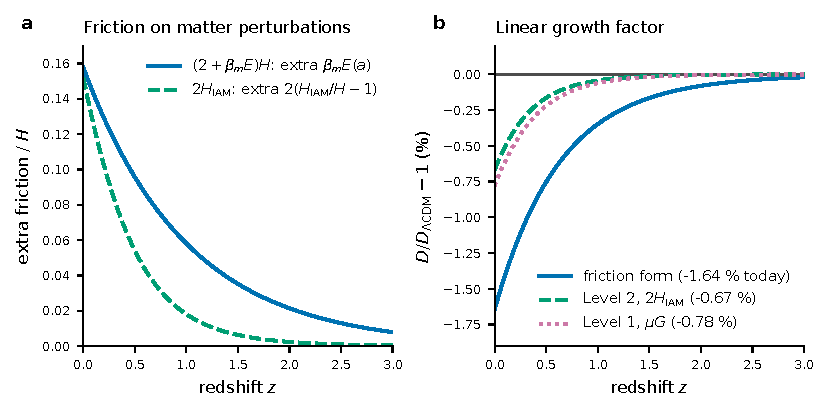
\includegraphics[width=\textwidth]{figures/part2/fig_eg_forms.pdf}
\caption[Three forms of the growth term]{The informational term in the growth equation, $\beta_m=\Omega_m/2$ fixed, $\Omega_m=0.3153$, same early amplitude.
(a) Extra friction on matter perturbations in units of $H$: $\beta_mE(a)$ in the friction form, Eq.~\eqref{eq:eg_growth}, and $2(H_{\rm IAM}/H-1)$ in the
Level~2 form. (b) The linear growth factor relative to $\Lambda$CDM: $-1.64\,\%$ today in the friction form, $-0.67\,\%$ in the Level~2 form and $-0.78\,\%$ in
the Level~1 effective-coupling form. Script \texttt{docs/book/figscripts/\allowbreak{}fig\_p2\_entropic\_gravity.py}. \calc}\label{fig:eg_forms}
\end{figure}

This is the origin of the dual-sector $\mu$--$\Sigma$ prediction. Massive particles travel on timelike paths; proper time elapses; gravitational
decoherence acts continuously. Photons travel on null geodesics; no proper time elapses; they are never subject to the decoherence process. \conjecture\
(decoherence eligibility, Section~\ref{sec:th:split}) The prediction $\Sigma=1$ (no change to the lensing response) follows from this geometric fact, not
from a parameter choice. The prediction $\mu<1$ follows from the matter-sector term. \derived\ (given the eligibility rule) $\mu<1$ is a weaker effective
coupling for matter: $1-\mu=13.62\,\%$ at $z=0$ is the coupling deficit, not the growth deficit. In the two chain forms the growth it produces is the $0.7$--$0.8\,\%$
in the linear growth factor above and a deficit in $f\sigma_8$ of $4.25\,\%$ at $z=0$, $2.17\,\%$ at $z=0.3$, $1.35\,\%$ at $z=0.5$ and $0.41\,\%$ at $z=1$
(Chapter~\ref{ch:virial}, Section~\ref{sec:vc_growth}). \calc

% ============================================================
\section{The coupling constant: \texorpdfstring{$\beta_m=\Omega_m/2$}{beta\_m = Omega\_m/2}}\label{sec:eg_coupling}
The coefficient $\beta_m$ is not a free parameter. It is derived from the virial theorem.

For any self-gravitating system bound by a $1/r$ interaction the derivation is short. Define the virial $\mathcal G=\sum_i\mathbf p_i\cdot\mathbf r_i$. Then
$d\mathcal G/dt=2T+\sum_i\mathbf F_i\cdot\mathbf r_i$. For a bound system $\mathcal G$ stays finite, so its long-time average derivative vanishes:
$2\langle T\rangle=-\langle\sum_i\mathbf F_i\cdot\mathbf r_i\rangle$. For an interaction energy homogeneous of degree $k$ in the coordinates, Euler's theorem gives
$\sum_i\mathbf r_i\cdot\nabla_iV=kV$, so $2\langle T\rangle=k\langle V\rangle$. For gravity $k=-1$:
\begin{equation}2\langle T\rangle+\langle V\rangle=0\quad\Longrightarrow\quad\langle T\rangle=\tfrac12|\langle V\rangle| .\label{eq:eg_virial}\end{equation}
\derived\ Exactly half the gravitational energy budget resides in kinetic degrees of freedom. In IAM the kinetic channel is the decoherence-producing
channel --- irreversible random motions of particles within collapsing structures generate the classical information requiring holographic encoding.
\conjecture\ (the identification) The informational energy density contribution is therefore $\Omega_m/2$, giving
\begin{equation}\beta_m=\frac{\Omega_m}{2}=0.15765\label{eq:eg_beta}\end{equation}
for $\Omega_m=0.3153$~\cite{Planck2018VI}. \derived\ (the factor $\tfrac12$) \calc\ (the number) The full argument, with the comparison against halo mass
functions, is Section~\ref{sec:th:coupling} and Chapter~\ref{ch:virial}.

The value is fixed before any data are used and held fixed, not fitted, in every chain of Chapters~\ref{ch:dual} and~\ref{ch:level2}; the chains therefore
test the amplitude it implies, not its value. Published simulations measure the halo virial ratio $2T/|U|$ within the virial radius at or slightly above
unity, about $1.15$ at $10^{12}\,h^{-1}M_\odot$ and $1.25$ at $10^{15}\,h^{-1}M_\odot$~\cite{Neto2007,Power2012} \observed; that ratio describes the dynamical
state of halos and is not a measurement of $\beta_m$. The test with existing data is the analysis with $\mu_0$ left free (Section~\ref{sec:chains}); future
growth data sharpen it. \prediction\ The same $\tfrac12$ partition holds from hydrogen atoms through stellar structure and galaxy clusters to the cosmic horizon --- 37 orders of
magnitude in physical scale, 33 of them from the atom to the cluster (Chapter~\ref{ch:virial_law}, Section~\ref{sec:vi_evidence}). The virial theorem is one instance of IAM's Law operating in every
domain.

% ============================================================
\section{The activation function \texorpdfstring{$E(a)$}{E(a)}}\label{sec:eg_activation}
$E(a)$ is derived by integrating the decoherence rate over cosmic history, weighted by the Gibbons--Hawking encoding temperature $T_H=H/2\pi$ and the
horizon area $A_H=4\pi/H^2$ (Section~\ref{sec:th:activation}). In the matter era the record written per e-fold scales as
$dS_{\rm info}/d\ln a\propto\rho_mD^nf/(T_HA_H)\propto a^{-3}a^n/(a^{-3/2}a^3)=a^{n-9/2}$; the decoherence integral requires $S_{\rm info}\propto-1/a$, which
fixes $n-9/2=-1$, $n=7/2$ (Section~\ref{sec:th:exponent}). \derived\ The first law for the informational piece, $-dE_{\rm info}=T_H\,dS_{\rm info}$, then
gives $\dot\rho_{\rm info}=\rho_{\rm info}H/a$ and $\rho_{\rm info}\propto\exp(C-1/a)$ (Eqs.~\eqref{eq:th:rhodot}--\eqref{eq:th:rhoint}). The result is
\begin{equation}E(a)=\exp\Big(1-\frac1a\Big).\label{eq:eg_Ea}\end{equation}
\derived

Within the family $\exp(C-k/a)$, two boundary conditions fix $E(a)$ completely without free parameters:
\begin{itemize}
\item $E(1)=1$: the present-day informational contribution is normalised to the matter energy density scale. This gives $C=k$.
\item $E(a)\to e$ as $a\to\infty$: the self-limiting nature of the feedback (expansion dilutes matter, slows decoherence) causes the cumulative entropy to
asymptote to a finite ceiling. This gives $C=1$.
\end{itemize}
\derived\ The two conditions give $C=k=1$; the exponent $n=7/2$ gives $k=1$ independently, so the ceiling $e$ is also a consequence of the derivation. With the full
$\Lambda$CDM background the accumulated record for $D^{7/2}$ is fitted by $\exp(0.93-1.02/a)$ (Section~\ref{sec:numerics}). \calc

At $a=1$ today, $E(1)/e=1/e\approx36.8\,\%$: the informational term stands at $36.8\,\%$ of its eventual ceiling. \calc\ Today is also the inflection point of
the activation function in $\ln a$, where the informational entropy production per e-fold of expansion, $dE/d\ln a=E/a$, is at its peak. Per unit cosmic
time the rate $dE/dt=HE/a$ peaked earlier, at $z=1.26$; per unit scale factor $dE/da=E/a^2$ peaks at $a=1/2$ (Chapter~\ref{ch:wzfuture}). \calc

% ============================================================
\section{Comparison with Barrow and Tsallis holographic cosmologies}\label{sec:eg_compare}
Table~\ref{tab:eg_compare} summarises the structural comparison. Both families of models emerge from the same thermodynamic-gravity conjecture. The key
difference is where new physics enters: in the entropy functional (Barrow, Tsallis) or in the entropy source term (IAM).

\begin{table}[htbp]
\centering\small
\caption{Structural comparison of entropy-based cosmological frameworks. Entries for IAM: Sections~\ref{sec:eg_lead}--\ref{sec:eg_activation} and
Chapter~\ref{ch:dual}. The $\mu$--$\Sigma$ entry for the deformed laws is structural: its value depends on how the deformation is carried into the
perturbation equations. \interp}\label{tab:eg_compare}
\renewcommand{\arraystretch}{1.3}
\begin{tabularx}{\linewidth}{@{}>{\raggedright\arraybackslash}p{2.7cm}>{\raggedright\arraybackslash}X>{\raggedright\arraybackslash}X@{}}
\toprule
Feature & Barrow / Tsallis holographic dark energy & IAM \\
\midrule
Foundation & Thermodynamic-gravity conjecture (Jacobson; Cai--Kim) & Same foundation \\
Modification & Entropy functional: $S_{\rm BH}\to S_{\rm Barrow}$ or $S_{\rm Tsallis}$ & Entropy source: $S_{\rm total}=S_{\rm BH}+S_{\rm info}$ \\
Free parameters & $\Delta$ (Barrow) or $\delta$ (Tsallis), fitted to data & None: $\beta_m=\Omega_m/2$ from the virial theorem \\
Background modified? & Yes: Friedmann equations altered & No: standard $\Lambda$CDM background \\
Perturbations modified? & Yes, through the modified Friedmann equations & Yes: a matter-sector term only \\
$\mu$--$\Sigma$ signature & Generally $\mu\neq1$, $\Sigma\neq1$ & $\mu<1$, $\Sigma=1$ exactly \\
$H_0$ & $72.2\pm0.9$ in one data combination; may ease the tension~\cite{Luciano2025} & Two sector rates: photon $67.16\pm0.47$ (Level~2 chain), matter
$67.16\sqrt{1+\beta_m}=72.26$ (output) \\
Information criteria vs.\ $\Lambda$CDM & $\Lambda$CDM slightly favoured (AIC, Bayes evidence)~\cite{Luciano2025} & No parameter added: $\Delta{\rm AIC}=\Delta\chi^2_{\min}=+0.54$ to
$+1.73$, the CMB reproduced with no added parameter \\
\bottomrule
\end{tabularx}
\end{table}

The information-criterion comparison deserves particular attention. Because Barrow and Tsallis cosmologies introduce one additional free parameter, the
Akaike criterion $\Delta{\rm AIC}=\Delta\chi^2_{\min}+2\Delta k$ penalises them by $2$ relative to $\Lambda$CDM even when the fit improves. IAM introduces
no additional free parameter --- $\beta_m$ is fully determined by $\Omega_m$, which is already a standard $\Lambda$CDM parameter. IAM therefore carries no
AIC penalty: its $\Delta{\rm AIC}$ equals its $\Delta\chi^2_{\min}$, $+0.54$ at Level~2 and $+0.56$ to $+1.73$ at Level~1 (Section~\ref{sec:chains}). \calc

% ============================================================
\section{A note on the entropy exponent}\label{sec:eg_exponent}
There is a natural question to ask of the Barrow--Tsallis framework: why does the entropy exponent take the value it does? The deformation parameters $\Delta$
and $\delta$ are physically motivated --- fractal horizon structure, non-extensive statistics --- but their values are not derived from first principles.
They are measured from data. \openprob

IAM suggests a perspective on an adjacent question. If $S_{\rm info}$ from decoherence is the correct physical source of the cosmological entropy
correction, then the apparent need for a non-standard entropy functional in other models may reflect an incomplete accounting of entropy sources rather
than a modification to the entropy--area law itself. Standard Bekenstein--Hawking entropy may be exact; the horizon entropy budget simply includes more
terms than previously recognised. \conjecture

Whether Barrow or Tsallis entropy captures genuine Planck-scale physics is an open question IAM does not resolve. \openprob\ The narrower point is that the
same late-time cosmological phenomenology that motivates entropy-modification approaches can be obtained from an entropy-source approach with zero free
parameters and a derivable coupling constant. \interp

% ============================================================
\section{Validation in Markov chains and the key predictions}\label{sec:eg_validation}
\subsection{Validation}
IAM has been tested against the Planck 2018 CMB likelihood through eighteen Markov chains (Section~\ref{sec:chains}): twelve at Level~1 through the MGCAMB
$\mu$--$\Sigma$ parametrisation; three at Level~2 through direct modification of CAMB's perturbation equations; two at Level~2b, placing the same term in the
background expansion instead, which drives $H_0$ to $61.45$ and $61.52$ and confirms that the mechanism belongs at the perturbation level; and one with the
baryon density left free (Chapter~\ref{ch:baryon}). Every chain's last recorded Gelman--Rubin $R-1$ is at or below $0.010$. \measured

\begin{table}[htbp]
\centering\small
\caption{Key IAM predictions and current observational status. Differences in units of the data error: $\mu_0$ $-0.80\sigma$ and $-0.82\sigma$; $\Sigma_0$
$-0.94\sigma$ and $-0.31\sigma$; $\sigma_8$ $-0.12\sigma$; matter-sector $H_0$ $-0.75\sigma$ (\texttt{verify\_entropic\_gravity.py}, section~7). \calc}\label{tab:eg_numbers}
\renewcommand{\arraystretch}{1.3}
\begin{tabularx}{\linewidth}{@{}l>{\raggedright\arraybackslash}p{3.6cm}>{\raggedright\arraybackslash}p{2.6cm}>{\raggedright\arraybackslash}X@{}}
\toprule
Quantity & IAM value & Current data & Source \\
\midrule
$\mu_0$ & $-0.136$ \derived & $0.04\pm0.22$ & DESI DR1 full shape + BAO, CMB, DES Y3~\cite{DESI2024VII} \\
 & & $0.02\pm0.19$ & ACT + WMAP + SDSS + SN~\cite{Andrade2024} \\
$\Sigma_0$ (deviation) & $0$ (null worldlines) \derived & $0.044\pm0.047$ & DESI DR1 full shape + BAO, CMB, DES Y3~\cite{DESI2024VII} \\
 & & $0.021\pm0.068$ & ACT + WMAP + SDSS + SN~\cite{Andrade2024} \\
$\sigma_8$ & $0.7998\pm0.0058$ (Level~2 chain; $\Lambda$CDM $0.8087$) \measured & $0.802^{+0.022}_{-0.018}$ & KiDS-Legacy + DES Y3 + DESI DR1 + Pantheon+~\cite{Stolzner2025} \\
$H_0^{\rm matter}$ & $72.26$\,km\,s$^{-1}$Mpc$^{-1}$ \calc & $73.04\pm1.04$ & SH0ES~\cite{Riess2022} \\
$\Delta\chi^2_{\min}$ & $+0.54$ (Level~2, Planck); $+0.56$ to $+1.73$ (Level~1) \measured & --- & eighteen Planck chains (Section~\ref{sec:chains}) \\
$\beta_m$ & $\Omega_m/2=0.15765$ \derived & fixed in every chain, not fitted & --- \\
\bottomrule
\end{tabularx}
\end{table}

\subsection{Falsifiable predictions}
IAM makes three near-term quantitative predictions.
\begin{enumerate}
\item \textbf{Euclid $\mu$--$\Sigma$ measurement.} The IAM prediction $\mu_0=-0.136$, $\Sigma_0=0$ is directly testable by Euclid. The combination $\mu<1$
with $\Sigma=1$ is the signature IAM predicts among viable models in the $\mu$--$\Sigma$ plane: in the quasi-static regime $f(R)$ gravity gives $\mu>1$ with
$\Sigma=1$~\cite{PogosianSilvestri2016}; the normal branch of DGP gives $\mu>1$; the self-accelerating branch of DGP shares $\mu<1$, $\Sigma=1$ but carries a
ghost~\cite{Koyama2007} and is in tension with CMB, supernova and $H_0$ data~\cite{Fang2008}; general Horndeski theories give $\Sigma\neq1$. The forecast is in Section~\ref{sec:sp_euclid}. \prediction
\item \textbf{The growth-rate trajectory.} The IAM $f\sigma_8(z)$ trajectory, suppressed by the matter-sector friction, is consistent with the DESI DR1
full-shape growth data without requiring $w<-1$: on the six bins $\chi^2$ is $5.24$ for IAM (MGCAMB form) against $4.51$ for $\Lambda$CDM
(Section~\ref{sec:vt_record}). \calc\ The interpretation proposed here is that the apparent phantom crossing at $z\approx0.35$--$0.5$ is a growth--geometry tension, not a
dark-energy signature. \conjecture\ The DESI DR2 preference for an evolving equation of state comes from distances alone (Section~\ref{sec:vt_phantom}), so the
test of that interpretation is the two-ruler comparison of Chapter~\ref{ch:sectortension}, together with a direct confrontation of the later DESI growth
measurements with the predicted trajectory. \openprob
\item \textbf{Galaxy cluster lensing-to-dynamics ratio.} The dual-sector structure predicts $M_{\rm lens}/M_{\rm dyn}=1/\mu(z)>1$ in a redshift-dependent
pattern that approaches unity at high $z$ as $\mu(a)\to1$: $1.158$ today, $1.105$ at $z=0.2$, $1.055$ at $0.5$, $1.018$ at $1$ and $1.002$ at $2$. \calc\ This is
qualitatively distinct from a constant hydrostatic bias and testable with eROSITA, Planck SZ and weak-lensing data in combination, with one mass method
throughout. \prediction\ The ratio holds in the Level~1 effective-coupling form; in the Level~2 form it is $1$ at every redshift, and which form applies
inside virialised clusters is open (Chapter~\ref{ch:lensdyn}, Section~\ref{sec:ld_hold}). \openprob
\end{enumerate}
If the growth surveys measure $\mu$ consistent with general relativity at a precision that excludes the IAM amplitude, IAM in this form is
ruled out; the decisive measurement is the turn-on of the growth ramp (Section~\ref{sec:sp_euclid}). \prediction

% ============================================================
\section{Summary}\label{sec:eg_summary}
The shared foundation is the Jacobson--Cai--Kim result: gravitational field equations are thermodynamic equations of state derivable from the first law
applied to the cosmic horizon.

IAM's specific contribution is to identify gravitational decoherence of collapsing matter as a physical source of additional horizon entropy. This source
term, built from Landauer's principle and the virial theorem, produces a matter-sector Hubble friction term with no free parameters. The coupling
$\beta_m=\Omega_m/2$ is fixed by the virial partition before any data are used and is held fixed in every chain.

The framework is consistent with the full Planck 2018 likelihood ($\Delta\chi^2=+0.54$ at Level~2), lowers $\sigma_8$ to $0.800$, $0.12\sigma$ from the joint
weak-lensing value, and places the two sector rates within $1\sigma$ of both Planck ($-0.37\sigma$) and SH0ES ($-0.75\sigma$) with no parameter
adjustment. It carries no AIC penalty because no new free parameter is introduced.

Euclid's $\mu$--$\Sigma$ measurement provides a direct test of the IAM prediction $\mu_0=-0.136$, $\Sigma_0=0$, forecast in
Section~\ref{sec:sp_euclid}. The derivation chain, the Markov chains, the modified CAMB Fortran source and the analysis scripts are in the repository.

Everything here can be rerun today from the repository. A cosmologist can set the comparison with the other entropic proposals against the same likelihood, and a relativist can take the $\mu$--$\Sigma$ test to the survey forecasts before the data arrive.

\section{Status of the results}
\providecommand{\lightrowrule}{\arrayrulecolor{black!25}\specialrule{0.3pt}{0pt}{0pt}\arrayrulecolor{black}}
\begin{center}\small\begin{tabularx}{\linewidth}{>{\raggedright\arraybackslash}Xl}\toprule
Result & Label\\\midrule
First law on the apparent horizon returns the Friedmann equations, Eqs.~\eqref{eq:eg_flux}--\eqref{eq:eg_friedmann} & \derived\\\lightrowrule
Field equations as thermodynamic equations of state & \interp\\\lightrowrule
$S_{\rm total}=S_{\rm BH}+S_{\rm info}$, Eq.~\eqref{eq:eg_stotal}; records encoded on the horizon & \conjecture\\\lightrowrule
Landauer cost $k_B\ln2$ per bit & \observed\\\lightrowrule
Growth equation in the friction form, Eqs.~\eqref{eq:eg_growth}--\eqref{eq:eg_growthN}; growth in the three forms & \derived\ \calc\\\lightrowrule
Decoherence eligibility (timelike worldlines only) & \conjecture\\\lightrowrule
$\Sigma=1$, $\mu<1$ given eligibility & \derived\\\lightrowrule
$2\langle T\rangle+\langle V\rangle=0$; the $\tfrac12$ partition & \derived\\\lightrowrule
Kinetic channel as the decoherence channel & \conjecture\\\lightrowrule
$\beta_m=\Omega_m/2=0.15765$ & \derived\ \calc\\\lightrowrule
$E(a)=\exp(1-1/a)$, $n=7/2$ & \derived\\\lightrowrule
Peak of the writing rate: per e-fold today, per unit time at $z=1.26$ & \calc\\\lightrowrule
Barrow and Tsallis constraints after DESI DR2 & \observed\\\lightrowrule
No AIC penalty; $\Delta{\rm AIC}=\Delta\chi^2_{\min}$ & \calc\\\lightrowrule
Bekenstein--Hawking entropy may be exact & \conjecture\\\lightrowrule
Chain results, Table~\ref{tab:eg_numbers} & \measured\\\lightrowrule
Euclid, growth trajectory, cluster ratio & \prediction\\\lightrowrule
Phantom crossing as growth--geometry tension & \conjecture\\\lightrowrule
Implementation form inside clusters; Planck-scale content of deformed laws & \openprob\\\bottomrule
\end{tabularx}\end{center}
